\section{Experiments}
\begin{frame}{Experiments}
	\tableofcontents[currentsection, currentsubsection, hideothersubsections]
\end{frame}

\subsection{Method}
\begin{frame}{Experiments}{Method}		
	\begin{columns}
		\begin{column}{0.5\textwidth}
			\begin{itemize}
				\item Design set-up
				\item Control and adjust equipment
				\item Perform the experiment
			\end{itemize}	
		\end{column}
		\begin{column}{0.5\textwidth} 
		\end{column}
	\end{columns}
\end{frame}

\begin{frame}{Experiments}{Control and Adjusting}		
	\begin{columns}
		\begin{column}{0.5\textwidth}
			\begin{itemize}
				\item Using a reference calibrator
				\item Yields a given dB @ calibrators frequency
				\item Record and examine signal
				\item Account for the difference 
			\end{itemize}	
		\end{column}	
		\begin{column}{0.5\textwidth} 
		\end{column}
	\end{columns}
\end{frame}

\subsection{Experiments in thie Project}
\begin{frame}{Experiments}{Listening Test}		
	\begin{columns}
		\begin{column}{0.5\textwidth}
			\begin{itemize}
				\item Determining threshold
				\item Using AAU students
				\item Results
				\begin{itemize}
					\item 10 dB attenuation is required
				\end{itemize}
			\end{itemize}	
		\end{column}	
		\begin{column}{0.5\textwidth} 
			\begin{figure}
					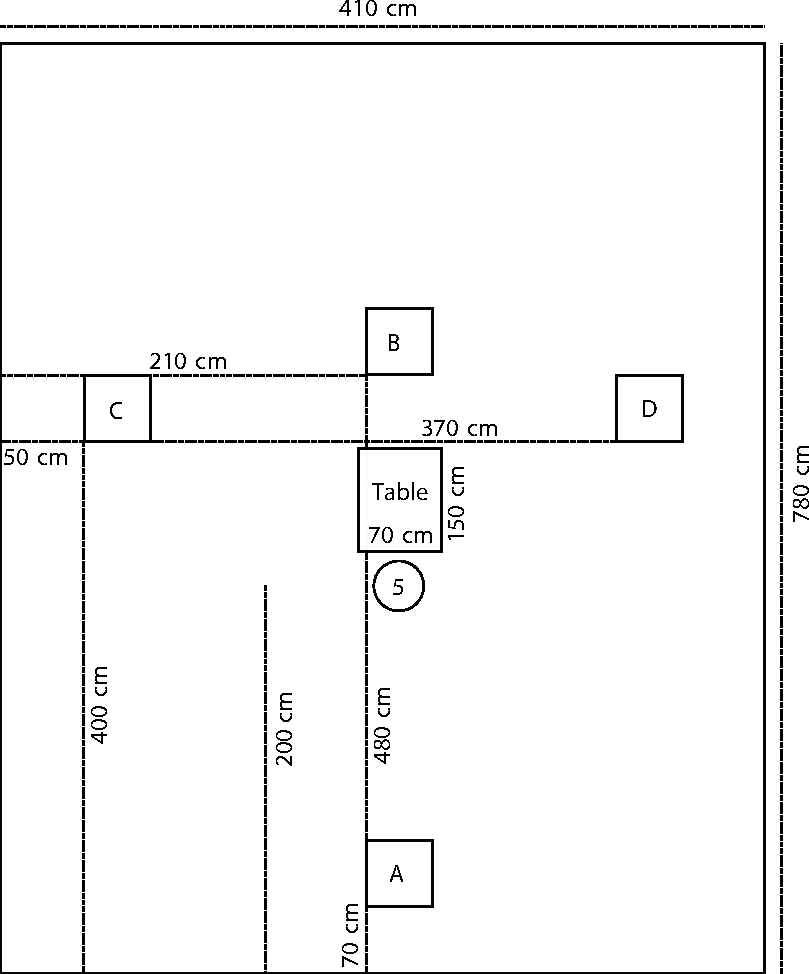
\includegraphics[width=1\textwidth]{figures/ListeningTestSetup.jpg}
			\end{figure}
		\end{column}
	\end{columns}
\end{frame}

\begin{frame}{Experiments}{Measuring a Transfer-Function (Headphone)}		
	\begin{columns}
		\begin{column}{0.5\textwidth}
			\begin{itemize}
				\item Headphone Transfer-function
				\begin{itemize}
					\item Physical cup of headphone
				\end{itemize}
				\item{Logarithmic Chirp}
				\item Transfer-function formula:
					\begin{equation*}
						H(f)=\frac{Y(f)}{X(f)}=\frac{\mathscr{F}(y(t))\times\mathscr{F}^{\ast}(x(t))}{\mathscr{F}(x(t))\times\mathscr{F}^{\ast}(x(t))}
					\end{equation*}
			\end{itemize}
		\end{column}
		\begin{column}{0.5\textwidth} 
			\begin{figure}[h]
				\includegraphics[width=1\textwidth]{figures/TransferFunctionHP}
			\end{figure}
		\end{column}
	\end{columns}
\end{frame}

\begin{frame}{Experiments}{Measuring a Transfer-Function (Headphone)}		
	\begin{columns}
		\begin{column}{0.3\textwidth}
			\begin{itemize}
				\item Results
				\begin{itemize}
					\item[\textcolor{MATLABorange}{---}] FFT of 960 coefficients
					\item[\textcolor{MATLABblue}{---}] FFT of 386,024 coefficients
				\end{itemize}
			\end{itemize}
		\end{column}
		\begin{column}{0.7\textwidth} 
			\begin{figure}[h]
				\input{figures/compfilterHP.tex}
			\end{figure}
		\end{column}
	\end{columns}
\end{frame}

\begin{frame}{Experiments}{Measuring a Transfer-Function (Cancellation Path)}		
	\begin{columns}
		\begin{column}{0.5\textwidth}
			\begin{itemize}
				\item Cancellation Path Transfer-function
				\begin{itemize}
					\item Headphone speaker \\ $\rightarrow$ Error microphone
				\end{itemize}
				\item{Logarithmic Chirp}
			\end{itemize}
		\end{column}
		\begin{column}{0.5\textwidth} 
			\begin{figure}[h]
				\includegraphics[width=1\textwidth]{figures/TransferFunctionCP}
			\end{figure}
		\end{column}
	\end{columns}
\end{frame}

\begin{frame}{Experiments}{Measuring a Transfer-Function (Cancellation Path)}		
	\begin{columns}
		\begin{column}{0.3\textwidth}
			\begin{itemize}
				\item Results
				\begin{itemize}
					\item[\textcolor{MATLABorange}{---}] FFT of 960 coefficients
					\item[\textcolor{MATLABblue}{---}] FFT of 480,256 coefficients
				\end{itemize}
			\end{itemize}
		\end{column}
		\begin{column}{0.7\textwidth} 
			\begin{figure}[h]
				% This file was created by matlab2tikz.
%
%The latest updates can be retrieved from
%  http://www.mathworks.com/matlabcentral/fileexchange/22022-matlab2tikz-matlab2tikz
%where you can also make suggestions and rate matlab2tikz.
%
\definecolor{mycolor1}{rgb}{0.00000,0.44700,0.74100}%
\definecolor{mycolor2}{rgb}{0.85000,0.32500,0.09800}%
%
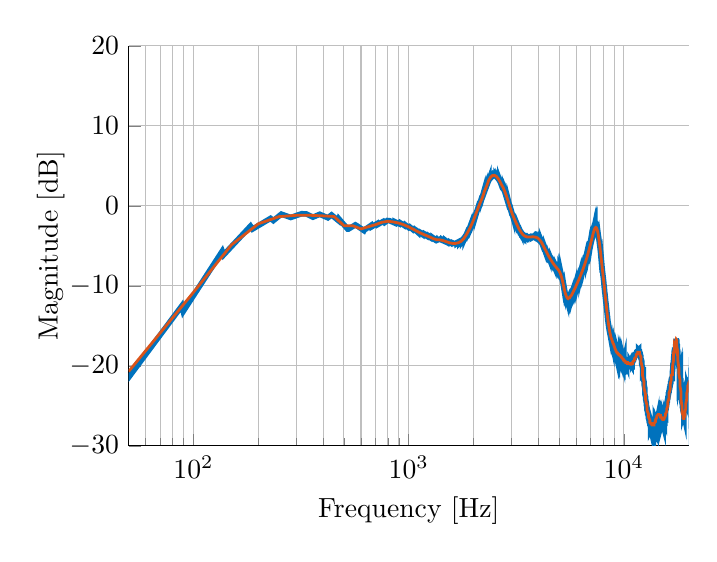
\begin{tikzpicture}

\begin{axis}[%
width=2.8in,
height=2in,
at={(1.457in,0.712in)},
scale only axis,
xmode=log,
xmin=50,
xmax=20000,
xminorticks=true,
xlabel={Frequency [Hz]},
xmajorgrids,
xminorgrids,
ylabel style={yshift=-0.5em},
%xlabel style={yshift=-0.2em},
ymin=-30,
ymax=20,
ylabel={Magnitude [dB]},
ymajorgrids,
axis background/.style={fill=white},
axis x line*=bottom,
axis y line*=left
]
\addplot [color=mycolor1,solid,forget plot, line width=2pt]
table[row sep=crcr]{%
	39.9	-24.3\\
	41.4	-24.4\\
	88.3	-12.5\\
	89.6	-13.2\\
	136	-5.67\\
	138	-6.14\\
	184	-2.53\\
	188	-2.91\\
	228	-1.57\\
	235	-1.85\\
	256	-1.04\\
	283	-1.46\\
	318	-0.988\\
	334	-1.01\\
	359	-1.42\\
	386	-1.06\\
	421	-1.5\\
	438	-1.14\\
	473	-1.88\\
	475	-1.67\\
	521	-2.92\\
	524	-2.92\\
	565	-2.38\\
	573	-2.47\\
	619	-3.09\\
	620	-3.05\\
	668	-2.45\\
	671	-2.64\\
	714	-2.21\\
	717	-2.35\\
	763	-1.94\\
	772	-2.1\\
	796	-1.84\\
	814	-1.86\\
	861	-2.15\\
	862	-1.98\\
	906	-2.27\\
	912	-2.12\\
	956	-2.48\\
	961	-2.36\\
	1e+03	-2.73\\
	1.01e+03	-2.63\\
	1.05e+03	-3.01\\
	1.06e+03	-2.9\\
	1.1e+03	-3.29\\
	1.1e+03	-3.18\\
	1.15e+03	-3.53\\
	1.15e+03	-3.43\\
	1.2e+03	-3.72\\
	1.2e+03	-3.62\\
	1.25e+03	-3.92\\
	1.25e+03	-3.82\\
	1.3e+03	-4.11\\
	1.3e+03	-4.01\\
	1.34e+03	-4.27\\
	1.35e+03	-4.17\\
	1.36e+03	-4.28\\
	1.39e+03	-4.17\\
	1.44e+03	-4.35\\
	1.44e+03	-4.25\\
	1.49e+03	-4.49\\
	1.49e+03	-4.38\\
	1.53e+03	-4.62\\
	1.54e+03	-4.5\\
	1.58e+03	-4.7\\
	1.59e+03	-4.6\\
	1.63e+03	-4.73\\
	1.64e+03	-4.73\\
	1.68e+03	-4.58\\
	1.68e+03	-4.68\\
	1.73e+03	-4.45\\
	1.73e+03	-4.56\\
	1.78e+03	-4.2\\
	1.78e+03	-4.3\\
	1.83e+03	-3.81\\
	1.83e+03	-3.91\\
	1.87e+03	-3.32\\
	1.88e+03	-3.41\\
	1.92e+03	-2.74\\
	1.92e+03	-2.83\\
	1.97e+03	-2.13\\
	1.97e+03	-2.22\\
	2.02e+03	-1.45\\
	2.02e+03	-1.5\\
	2.07e+03	-0.728\\
	2.07e+03	-0.781\\
	2.11e+03	-0.0306\\
	2.12e+03	-0.0878\\
	2.16e+03	0.637\\
	2.17e+03	0.578\\
	2.21e+03	1.34\\
	2.21e+03	1.26\\
	2.26e+03	2.05\\
	2.26e+03	1.99\\
	2.31e+03	2.63\\
	2.31e+03	2.59\\
	2.36e+03	3.27\\
	2.36e+03	3.21\\
	2.4e+03	3.65\\
	2.41e+03	3.58\\
	2.45e+03	3.85\\
	2.46e+03	3.77\\
	2.48e+03	3.88\\
	2.5e+03	3.85\\
	2.55e+03	3.64\\
	2.55e+03	3.72\\
	2.6e+03	3.4\\
	2.6e+03	3.46\\
	2.65e+03	3.07\\
	2.65e+03	3.12\\
	2.69e+03	2.64\\
	2.7e+03	2.7\\
	2.74e+03	2.28\\
	2.75e+03	2.35\\
	2.79e+03	1.79\\
	2.79e+03	1.86\\
	2.84e+03	1.26\\
	2.84e+03	1.28\\
	2.89e+03	0.657\\
	2.89e+03	0.687\\
	2.94e+03	0.0378\\
	2.94e+03	0.0693\\
	2.98e+03	-0.551\\
	2.99e+03	-0.504\\
	3.03e+03	-1.07\\
	3.03e+03	-1.03\\
	3.08e+03	-1.55\\
	3.08e+03	-1.51\\
	3.13e+03	-1.97\\
	3.13e+03	-1.93\\
	3.18e+03	-2.36\\
	3.18e+03	-2.32\\
	3.23e+03	-2.72\\
	3.23e+03	-2.67\\
	3.27e+03	-3.03\\
	3.28e+03	-2.99\\
	3.32e+03	-3.31\\
	3.32e+03	-3.26\\
	3.37e+03	-3.55\\
	3.37e+03	-3.49\\
	3.42e+03	-3.74\\
	3.42e+03	-3.68\\
	3.47e+03	-3.84\\
	3.47e+03	-3.78\\
	3.52e+03	-3.91\\
	3.52e+03	-3.85\\
	3.56e+03	-3.94\\
	3.57e+03	-3.88\\
	3.6e+03	-3.96\\
	3.62e+03	-3.95\\
	3.66e+03	-3.88\\
	3.67e+03	-3.95\\
	3.71e+03	-3.87\\
	3.72e+03	-3.87\\
	3.74e+03	-3.94\\
	3.77e+03	-3.87\\
	3.77e+03	-3.95\\
	3.81e+03	-3.88\\
	3.85e+03	-3.96\\
	3.86e+03	-3.9\\
	3.9e+03	-4\\
	3.91e+03	-3.94\\
	3.95e+03	-4.06\\
	3.95e+03	-4\\
	4e+03	-4.15\\
	4e+03	-4.1\\
	4.05e+03	-4.28\\
	4.05e+03	-4.25\\
	4.1e+03	-4.45\\
	4.1e+03	-4.42\\
	4.15e+03	-4.67\\
	4.15e+03	-4.62\\
	4.19e+03	-4.92\\
	4.2e+03	-4.87\\
	4.24e+03	-5.18\\
	4.24e+03	-5.13\\
	4.29e+03	-5.46\\
	4.29e+03	-5.41\\
	4.34e+03	-5.69\\
	4.34e+03	-5.65\\
	4.38e+03	-5.95\\
	4.39e+03	-5.88\\
	4.43e+03	-6.19\\
	4.44e+03	-6.15\\
	4.48e+03	-6.43\\
	4.48e+03	-6.37\\
	4.53e+03	-6.64\\
	4.53e+03	-6.6\\
	4.58e+03	-6.85\\
	4.58e+03	-6.8\\
	4.63e+03	-7.04\\
	4.63e+03	-6.98\\
	4.67e+03	-7.23\\
	4.68e+03	-7.16\\
	4.72e+03	-7.4\\
	4.72e+03	-7.34\\
	4.77e+03	-7.55\\
	4.78e+03	-7.49\\
	4.82e+03	-7.7\\
	4.82e+03	-7.64\\
	4.87e+03	-7.83\\
	4.87e+03	-7.77\\
	4.91e+03	-7.97\\
	4.92e+03	-7.9\\
	4.96e+03	-8.11\\
	4.97e+03	-8.05\\
	5.01e+03	-8.29\\
	5.02e+03	-8.23\\
	5.06e+03	-8.52\\
	5.06e+03	-8.46\\
	5.11e+03	-8.82\\
	5.11e+03	-8.76\\
	5.16e+03	-9.22\\
	5.16e+03	-9.14\\
	5.21e+03	-9.68\\
	5.21e+03	-9.63\\
	5.25e+03	-10.2\\
	5.26e+03	-10.1\\
	5.3e+03	-10.7\\
	5.31e+03	-10.6\\
	5.35e+03	-11.1\\
	5.35e+03	-11\\
	5.4e+03	-11.4\\
	5.4e+03	-11.3\\
	5.45e+03	-11.6\\
	5.45e+03	-11.5\\
	5.5e+03	-11.6\\
	5.52e+03	-11.6\\
	5.54e+03	-11.5\\
	5.55e+03	-11.6\\
	5.59e+03	-11.4\\
	5.6e+03	-11.5\\
	5.64e+03	-11.3\\
	5.64e+03	-11.4\\
	5.69e+03	-11.1\\
	5.69e+03	-11.2\\
	5.74e+03	-11\\
	5.74e+03	-11.1\\
	5.79e+03	-10.8\\
	5.79e+03	-10.9\\
	5.83e+03	-10.6\\
	5.84e+03	-10.7\\
	5.88e+03	-10.4\\
	5.88e+03	-10.5\\
	5.93e+03	-10.2\\
	5.93e+03	-10.3\\
	5.98e+03	-9.98\\
	5.98e+03	-10.1\\
	6.03e+03	-9.79\\
	6.03e+03	-9.87\\
	6.07e+03	-9.59\\
	6.08e+03	-9.66\\
	6.13e+03	-9.37\\
	6.13e+03	-9.45\\
	6.17e+03	-9.15\\
	6.17e+03	-9.24\\
	6.22e+03	-8.93\\
	6.22e+03	-9.02\\
	6.27e+03	-8.71\\
	6.27e+03	-8.79\\
	6.32e+03	-8.49\\
	6.32e+03	-8.57\\
	6.36e+03	-8.25\\
	6.37e+03	-8.34\\
	6.41e+03	-8.01\\
	6.42e+03	-8.12\\
	6.46e+03	-7.78\\
	6.47e+03	-7.87\\
	6.51e+03	-7.55\\
	6.51e+03	-7.63\\
	6.56e+03	-7.29\\
	6.56e+03	-7.38\\
	6.61e+03	-7.04\\
	6.61e+03	-7.13\\
	6.65e+03	-6.77\\
	6.66e+03	-6.87\\
	6.7e+03	-6.5\\
	6.71e+03	-6.59\\
	6.75e+03	-6.22\\
	6.76e+03	-6.31\\
	6.8e+03	-5.92\\
	6.8e+03	-6.02\\
	6.85e+03	-5.63\\
	6.85e+03	-5.72\\
	6.9e+03	-5.33\\
	6.9e+03	-5.42\\
	6.94e+03	-5\\
	6.95e+03	-5.1\\
	6.99e+03	-4.68\\
	7e+03	-4.78\\
	7.04e+03	-4.36\\
	7.04e+03	-4.46\\
	7.09e+03	-4.05\\
	7.09e+03	-4.14\\
	7.14e+03	-3.74\\
	7.14e+03	-3.82\\
	7.19e+03	-3.43\\
	7.19e+03	-3.51\\
	7.24e+03	-3.15\\
	7.24e+03	-3.24\\
	7.28e+03	-2.92\\
	7.29e+03	-3\\
	7.33e+03	-2.75\\
	7.33e+03	-2.82\\
	7.38e+03	-2.65\\
	7.39e+03	-2.74\\
	7.41e+03	-2.64\\
	7.43e+03	-2.66\\
	7.47e+03	-2.85\\
	7.48e+03	-2.79\\
	7.53e+03	-3.09\\
	7.53e+03	-3.03\\
	7.57e+03	-3.43\\
	7.58e+03	-3.38\\
	7.62e+03	-3.87\\
	7.62e+03	-3.82\\
	7.67e+03	-4.38\\
	7.67e+03	-4.35\\
	7.72e+03	-4.99\\
	7.72e+03	-4.95\\
	7.77e+03	-5.63\\
	7.77e+03	-5.58\\
	7.81e+03	-6.28\\
	7.82e+03	-6.22\\
	7.86e+03	-6.93\\
	7.87e+03	-6.9\\
	7.91e+03	-7.58\\
	7.91e+03	-7.57\\
	7.96e+03	-8.27\\
	7.96e+03	-8.24\\
	8.01e+03	-8.93\\
	8.01e+03	-8.88\\
	8.06e+03	-9.57\\
	8.06e+03	-9.52\\
	8.1e+03	-10.2\\
	8.11e+03	-10.2\\
	8.15e+03	-10.9\\
	8.15e+03	-10.8\\
	8.2e+03	-11.5\\
	8.2e+03	-11.5\\
	8.25e+03	-12.2\\
	8.25e+03	-12.1\\
	8.3e+03	-12.8\\
	8.3e+03	-12.8\\
	8.35e+03	-13.4\\
	8.35e+03	-13.4\\
	8.39e+03	-14\\
	8.4e+03	-14\\
	8.44e+03	-14.6\\
	8.44e+03	-14.6\\
	8.49e+03	-15.1\\
	8.49e+03	-15.1\\
	8.54e+03	-15.5\\
	8.54e+03	-15.5\\
	8.59e+03	-15.9\\
	8.59e+03	-15.9\\
	8.64e+03	-16.2\\
	8.64e+03	-16.2\\
	8.68e+03	-16.5\\
	8.69e+03	-16.4\\
	8.73e+03	-16.7\\
	8.73e+03	-16.7\\
	8.78e+03	-17\\
	8.78e+03	-16.9\\
	8.83e+03	-17.1\\
	8.83e+03	-17.1\\
	8.88e+03	-17.3\\
	8.88e+03	-17.2\\
	8.92e+03	-17.5\\
	8.93e+03	-17.4\\
	8.97e+03	-17.7\\
	8.98e+03	-17.6\\
	9.02e+03	-17.9\\
	9.02e+03	-17.8\\
	9.07e+03	-18\\
	9.07e+03	-18\\
	9.12e+03	-18.2\\
	9.12e+03	-18.1\\
	9.17e+03	-18.4\\
	9.17e+03	-18.3\\
	9.21e+03	-18.5\\
	9.22e+03	-18.4\\
	9.26e+03	-18.6\\
	9.27e+03	-18.5\\
	9.31e+03	-18.7\\
	9.31e+03	-18.6\\
	9.36e+03	-18.7\\
	9.36e+03	-18.6\\
	9.4e+03	-18.8\\
	9.41e+03	-18.7\\
	9.46e+03	-18.8\\
	9.48e+03	-18.7\\
	9.5e+03	-18.9\\
	9.51e+03	-18.8\\
	9.55e+03	-18.9\\
	9.56e+03	-18.8\\
	9.6e+03	-19\\
	9.61e+03	-18.9\\
	9.65e+03	-19\\
	9.65e+03	-18.9\\
	9.69e+03	-19.1\\
	9.7e+03	-19\\
	9.74e+03	-19.2\\
	9.75e+03	-19\\
	9.8e+03	-19.2\\
	9.8e+03	-19.1\\
	9.84e+03	-19.3\\
	9.84e+03	-19.2\\
	9.89e+03	-19.4\\
	9.89e+03	-19.2\\
	9.94e+03	-19.5\\
	9.94e+03	-19.3\\
	9.98e+03	-19.5\\
	1e+04	-19.4\\
	1e+04	-19.6\\
	1e+04	-19.4\\
	1.01e+04	-19.6\\
	1.01e+04	-19.4\\
	1.01e+04	-19.7\\
	1.01e+04	-19.5\\
	1.02e+04	-19.7\\
	1.02e+04	-19.5\\
	1.02e+04	-19.8\\
	1.02e+04	-19.5\\
	1.03e+04	-19.8\\
	1.03e+04	-19.8\\
	1.03e+04	-19.5\\
	1.04e+04	-19.5\\
	1.04e+04	-19.8\\
	1.04e+04	-19.8\\
	1.04e+04	-19.6\\
	1.05e+04	-19.6\\
	1.05e+04	-19.8\\
	1.05e+04	-19.6\\
	1.05e+04	-19.8\\
	1.05e+04	-19.6\\
	1.05e+04	-19.8\\
	1.06e+04	-19.6\\
	1.06e+04	-19.8\\
	1.06e+04	-19.6\\
	1.06e+04	-19.8\\
	1.07e+04	-19.6\\
	1.07e+04	-19.8\\
	1.07e+04	-19.8\\
	1.07e+04	-19.6\\
	1.08e+04	-19.8\\
	1.08e+04	-19.6\\
	1.08e+04	-19.8\\
	1.08e+04	-19.6\\
	1.09e+04	-19.7\\
	1.09e+04	-19.5\\
	1.09e+04	-19.6\\
	1.1e+04	-19.5\\
	1.1e+04	-19.6\\
	1.1e+04	-19.4\\
	1.1e+04	-19.5\\
	1.11e+04	-19.3\\
	1.11e+04	-19.4\\
	1.11e+04	-19.2\\
	1.11e+04	-19.3\\
	1.11e+04	-19.1\\
	1.11e+04	-19.2\\
	1.12e+04	-19\\
	1.12e+04	-19.1\\
	1.12e+04	-18.9\\
	1.12e+04	-18.9\\
	1.13e+04	-18.8\\
	1.13e+04	-18.8\\
	1.13e+04	-18.6\\
	1.13e+04	-18.7\\
	1.14e+04	-18.5\\
	1.14e+04	-18.5\\
	1.14e+04	-18.4\\
	1.14e+04	-18.4\\
	1.15e+04	-18.3\\
	1.15e+04	-18.3\\
	1.15e+04	-18.2\\
	1.15e+04	-18.2\\
	1.16e+04	-18.1\\
	1.16e+04	-18.2\\
	1.16e+04	-18\\
	1.16e+04	-18.1\\
	1.17e+04	-18\\
	1.17e+04	-18.1\\
	1.17e+04	-18\\
	1.17e+04	-18\\
	1.18e+04	-18.1\\
	1.18e+04	-18.1\\
	1.18e+04	-18.2\\
	1.18e+04	-18.2\\
	1.19e+04	-18.4\\
	1.19e+04	-18.3\\
	1.19e+04	-18.5\\
	1.19e+04	-18.5\\
	1.2e+04	-18.8\\
	1.2e+04	-18.7\\
	1.2e+04	-19.1\\
	1.2e+04	-19.1\\
	1.21e+04	-19.4\\
	1.21e+04	-19.4\\
	1.21e+04	-19.8\\
	1.21e+04	-19.8\\
	1.22e+04	-20.2\\
	1.22e+04	-20.2\\
	1.22e+04	-20.7\\
	1.22e+04	-20.6\\
	1.22e+04	-21.1\\
	1.23e+04	-21\\
	1.23e+04	-21.5\\
	1.23e+04	-21.5\\
	1.24e+04	-22\\
	1.24e+04	-21.9\\
	1.24e+04	-22.4\\
	1.24e+04	-22.3\\
	1.25e+04	-22.8\\
	1.25e+04	-22.7\\
	1.25e+04	-23.2\\
	1.25e+04	-23.1\\
	1.25e+04	-23.6\\
	1.25e+04	-23.5\\
	1.26e+04	-23.9\\
	1.26e+04	-23.8\\
	1.26e+04	-24.2\\
	1.26e+04	-24.1\\
	1.27e+04	-24.6\\
	1.27e+04	-24.5\\
	1.27e+04	-24.9\\
	1.27e+04	-24.8\\
	1.28e+04	-25.3\\
	1.28e+04	-25.2\\
	1.28e+04	-25.6\\
	1.28e+04	-25.5\\
	1.29e+04	-25.9\\
	1.29e+04	-25.8\\
	1.29e+04	-26.2\\
	1.29e+04	-26\\
	1.3e+04	-26.4\\
	1.3e+04	-26.3\\
	1.3e+04	-26.7\\
	1.3e+04	-26.5\\
	1.31e+04	-26.9\\
	1.31e+04	-26.7\\
	1.31e+04	-27.1\\
	1.31e+04	-27\\
	1.32e+04	-27.3\\
	1.32e+04	-27.1\\
	1.32e+04	-27.5\\
	1.32e+04	-27.3\\
	1.33e+04	-27.6\\
	1.33e+04	-27.4\\
	1.33e+04	-27.7\\
	1.33e+04	-27.5\\
	1.33e+04	-27.8\\
	1.34e+04	-27.6\\
	1.34e+04	-27.9\\
	1.34e+04	-27.6\\
	1.35e+04	-27.9\\
	1.35e+04	-27.7\\
	1.35e+04	-28\\
	1.35e+04	-27.8\\
	1.36e+04	-28\\
	1.36e+04	-27.8\\
	1.36e+04	-28.1\\
	1.36e+04	-27.8\\
	1.37e+04	-28.1\\
	1.37e+04	-28.1\\
	1.37e+04	-27.9\\
	1.37e+04	-28.2\\
	1.37e+04	-27.9\\
	1.38e+04	-27.8\\
	1.38e+04	-28.1\\
	1.38e+04	-28.2\\
	1.38e+04	-27.8\\
	1.39e+04	-28\\
	1.39e+04	-27.8\\
	1.39e+04	-28\\
	1.39e+04	-27.6\\
	1.39e+04	-27.9\\
	1.4e+04	-27.6\\
	1.4e+04	-27.8\\
	1.4e+04	-27.4\\
	1.41e+04	-27.7\\
	1.41e+04	-27.3\\
	1.41e+04	-27.6\\
	1.41e+04	-27.2\\
	1.41e+04	-27.5\\
	1.42e+04	-27.1\\
	1.42e+04	-27.3\\
	1.42e+04	-27\\
	1.43e+04	-27.2\\
	1.43e+04	-26.9\\
	1.43e+04	-27.2\\
	1.43e+04	-26.9\\
	1.43e+04	-27.1\\
	1.44e+04	-26.8\\
	1.44e+04	-27\\
	1.44e+04	-26.7\\
	1.45e+04	-26.8\\
	1.45e+04	-27.1\\
	1.45e+04	-27.1\\
	1.45e+04	-26.7\\
	1.45e+04	-27.1\\
	1.46e+04	-26.8\\
	1.46e+04	-26.8\\
	1.46e+04	-27\\
	1.46e+04	-27.2\\
	1.47e+04	-26.8\\
	1.47e+04	-26.8\\
	1.47e+04	-27.1\\
	1.47e+04	-27.2\\
	1.47e+04	-26.9\\
	1.48e+04	-26.9\\
	1.48e+04	-27.2\\
	1.48e+04	-27.2\\
	1.49e+04	-26.9\\
	1.49e+04	-27\\
	1.49e+04	-27.3\\
	1.49e+04	-27\\
	1.49e+04	-27.3\\
	1.5e+04	-27\\
	1.5e+04	-27.3\\
	1.5e+04	-27.1\\
	1.5e+04	-27.3\\
	1.51e+04	-27.3\\
	1.51e+04	-27.1\\
	1.51e+04	-27\\
	1.52e+04	-27.3\\
	1.52e+04	-27.3\\
	1.52e+04	-27\\
	1.52e+04	-27.2\\
	1.52e+04	-27\\
	1.53e+04	-27.1\\
	1.53e+04	-26.9\\
	1.53e+04	-27\\
	1.53e+04	-26.7\\
	1.54e+04	-26.9\\
	1.54e+04	-26.5\\
	1.54e+04	-26.7\\
	1.54e+04	-26.4\\
	1.55e+04	-26.5\\
	1.55e+04	-26.2\\
	1.55e+04	-26.3\\
	1.55e+04	-26\\
	1.56e+04	-26.1\\
	1.56e+04	-25.8\\
	1.56e+04	-25.9\\
	1.56e+04	-25.5\\
	1.56e+04	-25.8\\
	1.57e+04	-25.3\\
	1.57e+04	-25.5\\
	1.57e+04	-25.1\\
	1.57e+04	-25.4\\
	1.58e+04	-24.8\\
	1.58e+04	-25.1\\
	1.58e+04	-24.7\\
	1.58e+04	-24.9\\
	1.59e+04	-24.4\\
	1.59e+04	-24.6\\
	1.59e+04	-24.2\\
	1.59e+04	-24.4\\
	1.6e+04	-24\\
	1.6e+04	-24.2\\
	1.6e+04	-23.8\\
	1.6e+04	-24\\
	1.61e+04	-23.6\\
	1.61e+04	-23.8\\
	1.61e+04	-23.3\\
	1.61e+04	-23.6\\
	1.62e+04	-23.1\\
	1.62e+04	-23.4\\
	1.62e+04	-23\\
	1.62e+04	-23.2\\
	1.63e+04	-22.8\\
	1.63e+04	-23\\
	1.63e+04	-22.6\\
	1.63e+04	-22.9\\
	1.64e+04	-22.4\\
	1.64e+04	-22.7\\
	1.64e+04	-22.3\\
	1.64e+04	-22.5\\
	1.65e+04	-22.1\\
	1.65e+04	-22.3\\
	1.65e+04	-21.9\\
	1.65e+04	-22.1\\
	1.66e+04	-21.7\\
	1.66e+04	-21.9\\
	1.66e+04	-21.5\\
	1.66e+04	-21.8\\
	1.67e+04	-21.4\\
	1.67e+04	-21.7\\
	1.67e+04	-21.4\\
	1.67e+04	-21.4\\
	1.67e+04	-21.6\\
	1.68e+04	-21.6\\
	1.68e+04	-21.1\\
	1.68e+04	-21.3\\
	1.68e+04	-20.6\\
	1.68e+04	-20.8\\
	1.69e+04	-20.1\\
	1.69e+04	-20.3\\
	1.69e+04	-19.7\\
	1.69e+04	-19.9\\
	1.7e+04	-19.3\\
	1.7e+04	-19.5\\
	1.7e+04	-18.9\\
	1.7e+04	-19.1\\
	1.71e+04	-18.5\\
	1.71e+04	-18.7\\
	1.71e+04	-18.1\\
	1.71e+04	-18.3\\
	1.72e+04	-17.9\\
	1.72e+04	-18.1\\
	1.72e+04	-17.8\\
	1.72e+04	-17.7\\
	1.73e+04	-18.1\\
	1.73e+04	-17.9\\
	1.73e+04	-18.4\\
	1.73e+04	-18.4\\
	1.74e+04	-17.9\\
	1.74e+04	-18.2\\
	1.74e+04	-17.3\\
	1.74e+04	-17.5\\
	1.75e+04	-16.8\\
	1.75e+04	-17\\
	1.75e+04	-16.7\\
	1.75e+04	-16.6\\
	1.76e+04	-17\\
	1.76e+04	-16.7\\
	1.76e+04	-17.2\\
	1.76e+04	-17\\
	1.77e+04	-17.6\\
	1.77e+04	-17.3\\
	1.77e+04	-18\\
	1.77e+04	-17.7\\
	1.78e+04	-18.4\\
	1.78e+04	-18.1\\
	1.78e+04	-18.8\\
	1.78e+04	-18.5\\
	1.79e+04	-19.2\\
	1.79e+04	-18.9\\
	1.79e+04	-19.5\\
	1.79e+04	-19.3\\
	1.8e+04	-19.9\\
	1.8e+04	-19.6\\
	1.8e+04	-20.2\\
	1.8e+04	-19.9\\
	1.81e+04	-20.5\\
	1.81e+04	-20.3\\
	1.81e+04	-20.9\\
	1.81e+04	-20.6\\
	1.81e+04	-21.2\\
	1.82e+04	-20.9\\
	1.82e+04	-21.5\\
	1.82e+04	-21.2\\
	1.82e+04	-21.8\\
	1.83e+04	-21.5\\
	1.83e+04	-22.1\\
	1.83e+04	-21.9\\
	1.83e+04	-22.5\\
	1.83e+04	-22.2\\
	1.84e+04	-22.9\\
	1.84e+04	-22.6\\
	1.84e+04	-23.3\\
	1.84e+04	-23\\
	1.85e+04	-23.7\\
	1.85e+04	-23.4\\
	1.85e+04	-24\\
	1.85e+04	-23.9\\
	1.86e+04	-24.4\\
	1.86e+04	-24.2\\
	1.86e+04	-24.7\\
	1.86e+04	-24.5\\
	1.87e+04	-25\\
	1.87e+04	-24.8\\
	1.87e+04	-25.3\\
	1.87e+04	-25\\
	1.88e+04	-25.5\\
	1.88e+04	-25.3\\
	1.88e+04	-25.7\\
	1.88e+04	-25.5\\
	1.89e+04	-25.8\\
	1.89e+04	-25.5\\
	1.89e+04	-25.8\\
	1.89e+04	-25.9\\
	1.89e+04	-25.6\\
	1.9e+04	-25.9\\
	1.9e+04	-25.6\\
	1.9e+04	-25.8\\
	1.91e+04	-25.6\\
	1.91e+04	-25.8\\
	1.91e+04	-25.5\\
	1.91e+04	-25.4\\
	1.91e+04	-25.7\\
	1.92e+04	-25.6\\
	1.92e+04	-25.3\\
	1.92e+04	-25.5\\
	1.93e+04	-25.1\\
	1.93e+04	-25.3\\
	1.93e+04	-24.8\\
	1.93e+04	-25.1\\
	1.94e+04	-24.7\\
	1.94e+04	-24.9\\
	1.94e+04	-24.5\\
	1.94e+04	-24.7\\
	1.94e+04	-24.3\\
	1.95e+04	-24.5\\
	1.95e+04	-24.1\\
	1.95e+04	-24.3\\
	1.95e+04	-23.9\\
	1.96e+04	-24.1\\
	1.96e+04	-23.7\\
	1.96e+04	-23.8\\
	1.96e+04	-23.5\\
	1.97e+04	-23.6\\
	1.97e+04	-23.3\\
	1.97e+04	-23.5\\
	1.97e+04	-23.2\\
	1.97e+04	-23.3\\
	1.98e+04	-23\\
	1.98e+04	-23.3\\
	1.98e+04	-22.9\\
	1.99e+04	-23.1\\
	1.99e+04	-22.9\\
	1.99e+04	-23\\
	1.99e+04	-22.8\\
	2e+04	-22.7\\
	2e+04	-23\\
	2e+04	-22.6\\
	2e+04	-23.1\\
	2.01e+04	-23.2\\
	2.01e+04	-22.4\\
	2.01e+04	-22.5\\
	2.01e+04	-23.6\\
	2.02e+04	-23.8\\
	2.02e+04	-21.9\\
	2.02e+04	-24.1\\
	2.02e+04	-22.1\\
	2.02e+04	-24.2\\
	2.03e+04	-21.9\\
	2.03e+04	-22.1\\
	2.03e+04	-24.6\\
	2.03e+04	-25.1\\
	2.03e+04	-21.8\\
	2.04e+04	-21.4\\
	2.04e+04	-25.1\\
	2.04e+04	-25.7\\
	2.05e+04	-20.1\\
	2.05e+04	-20.7\\
	2.05e+04	-27.2\\
	2.06e+04	-28.4\\
	2.06e+04	-20.6\\
	2.06e+04	-18.9\\
	2.06e+04	-26.9\\
	2.06e+04	-19.9\\
	2.06e+04	-32.7\\
	2.07e+04	-26.7\\
	2.07e+04	-18.8\\
	2.07e+04	-39.7\\
	2.07e+04	-19.4\\
	2.08e+04	-29.9\\
	2.08e+04	-19.8\\
	2.08e+04	-34\\
	2.09e+04	-17.1\\
	2.09e+04	-32.1\\
	2.09e+04	-16.6\\
	2.09e+04	-16.6\\
	2.09e+04	-31\\
	2.1e+04	-22.6\\
};
\addplot [color=mycolor2,solid,forget plot, line width=1pt]
table[row sep=crcr]{%
	0	-57.4\\
	50	-20.7\\
	100	-10.8\\
	150	-4.89\\
	200	-2.25\\
	250	-1.35\\
	300	-1.19\\
	350	-1.19\\
	400	-1.26\\
	450	-1.33\\
	500	-2.48\\
	550	-2.5\\
	600	-2.89\\
	650	-2.61\\
	700	-2.36\\
	750	-2.06\\
	800	-1.93\\
	850	-2.02\\
	900	-2.16\\
	950	-2.38\\
	1e+03	-2.64\\
	1.05e+03	-2.93\\
	1.1e+03	-3.22\\
	1.15e+03	-3.48\\
	1.2e+03	-3.69\\
	1.25e+03	-3.89\\
	1.3e+03	-4.1\\
	1.35e+03	-4.24\\
	1.4e+03	-4.26\\
	1.45e+03	-4.36\\
	1.5e+03	-4.5\\
	1.55e+03	-4.63\\
	1.6e+03	-4.7\\
	1.65e+03	-4.7\\
	1.7e+03	-4.62\\
	1.75e+03	-4.45\\
	1.8e+03	-4.11\\
	1.85e+03	-3.64\\
	1.9e+03	-3.09\\
	1.95e+03	-2.48\\
	2e+03	-1.79\\
	2.05e+03	-1.03\\
	2.1e+03	-0.297\\
	2.15e+03	0.416\\
	2.2e+03	1.03\\
	2.25e+03	1.85\\
	2.3e+03	2.45\\
	2.35e+03	3.15\\
	2.4e+03	3.57\\
	2.45e+03	3.79\\
	2.5e+03	3.81\\
	2.55e+03	3.69\\
	2.6e+03	3.42\\
	2.65e+03	3.07\\
	2.7e+03	2.63\\
	2.75e+03	2.25\\
	2.8e+03	1.73\\
	2.85e+03	1.16\\
	2.9e+03	0.528\\
	2.95e+03	-0.11\\
	3e+03	-0.701\\
	3.05e+03	-1.22\\
	3.1e+03	-1.68\\
	3.15e+03	-2.1\\
	3.2e+03	-2.49\\
	3.25e+03	-2.85\\
	3.3e+03	-3.15\\
	3.35e+03	-3.41\\
	3.4e+03	-3.62\\
	3.45e+03	-3.76\\
	3.5e+03	-3.84\\
	3.55e+03	-3.89\\
	3.6e+03	-3.9\\
	3.65e+03	-3.9\\
	3.7e+03	-3.89\\
	3.75e+03	-3.88\\
	3.8e+03	-3.88\\
	3.85e+03	-3.9\\
	3.9e+03	-3.93\\
	3.95e+03	-3.99\\
	4e+03	-4.09\\
	4.05e+03	-4.23\\
	4.1e+03	-4.41\\
	4.15e+03	-4.62\\
	4.2e+03	-4.88\\
	4.25e+03	-5.16\\
	4.3e+03	-5.43\\
	4.35e+03	-5.68\\
	4.4e+03	-5.94\\
	4.45e+03	-6.2\\
	4.5e+03	-6.43\\
	4.55e+03	-6.65\\
	4.6e+03	-6.85\\
	4.65e+03	-7.05\\
	4.7e+03	-7.23\\
	4.75e+03	-7.41\\
	4.8e+03	-7.56\\
	4.85e+03	-7.7\\
	4.9e+03	-7.84\\
	4.95e+03	-7.99\\
	5e+03	-8.16\\
	5.05e+03	-8.39\\
	5.1e+03	-8.69\\
	5.15e+03	-9.08\\
	5.2e+03	-9.56\\
	5.25e+03	-10.1\\
	5.3e+03	-10.6\\
	5.35e+03	-11\\
	5.4e+03	-11.3\\
	5.45e+03	-11.5\\
	5.5e+03	-11.6\\
	5.55e+03	-11.5\\
	5.6e+03	-11.5\\
	5.65e+03	-11.3\\
	5.7e+03	-11.2\\
	5.75e+03	-11\\
	5.8e+03	-10.8\\
	5.85e+03	-10.6\\
	5.9e+03	-10.4\\
	5.95e+03	-10.2\\
	6e+03	-9.96\\
	6.05e+03	-9.75\\
	6.1e+03	-9.54\\
	6.15e+03	-9.32\\
	6.2e+03	-9.1\\
	6.25e+03	-8.88\\
	6.3e+03	-8.65\\
	6.35e+03	-8.41\\
	6.4e+03	-8.18\\
	6.45e+03	-7.94\\
	6.5e+03	-7.69\\
	6.55e+03	-7.43\\
	6.6e+03	-7.17\\
	6.65e+03	-6.9\\
	6.7e+03	-6.62\\
	6.75e+03	-6.33\\
	6.8e+03	-6.03\\
	6.85e+03	-5.72\\
	6.9e+03	-5.4\\
	6.95e+03	-5.07\\
	7e+03	-4.74\\
	7.05e+03	-4.41\\
	7.1e+03	-4.07\\
	7.15e+03	-3.75\\
	7.2e+03	-3.43\\
	7.25e+03	-3.15\\
	7.3e+03	-2.92\\
	7.35e+03	-2.77\\
	7.4e+03	-2.7\\
	7.45e+03	-2.75\\
	7.5e+03	-2.93\\
	7.55e+03	-3.22\\
	7.6e+03	-3.63\\
	7.65e+03	-4.14\\
	7.7e+03	-4.72\\
	7.75e+03	-5.35\\
	7.8e+03	-6.01\\
	7.85e+03	-6.69\\
	7.9e+03	-7.37\\
	7.95e+03	-8.05\\
	8e+03	-8.73\\
	8.05e+03	-9.39\\
	8.1e+03	-10\\
	8.15e+03	-10.7\\
	8.2e+03	-11.4\\
	8.25e+03	-12\\
	8.3e+03	-12.7\\
	8.35e+03	-13.4\\
	8.4e+03	-14\\
	8.45e+03	-14.5\\
	8.5e+03	-15\\
	8.55e+03	-15.4\\
	8.6e+03	-15.8\\
	8.65e+03	-16.1\\
	8.7e+03	-16.4\\
	8.75e+03	-16.6\\
	8.8e+03	-16.8\\
	8.85e+03	-17\\
	8.9e+03	-17.2\\
	8.95e+03	-17.3\\
	9e+03	-17.5\\
	9.05e+03	-17.7\\
	9.1e+03	-17.9\\
	9.15e+03	-18\\
	9.2e+03	-18.2\\
	9.25e+03	-18.3\\
	9.3e+03	-18.4\\
	9.35e+03	-18.4\\
	9.4e+03	-18.5\\
	9.45e+03	-18.6\\
	9.5e+03	-18.6\\
	9.55e+03	-18.7\\
	9.6e+03	-18.7\\
	9.65e+03	-18.8\\
	9.7e+03	-18.9\\
	9.75e+03	-18.9\\
	9.8e+03	-19\\
	9.85e+03	-19.1\\
	9.9e+03	-19.2\\
	9.95e+03	-19.2\\
	1e+04	-19.3\\
	1.00e+04	-19.4\\
	1.01e+04	-19.4\\
	1.02e+04	-19.5\\
	1.02e+04	-19.5\\
	1.02e+04	-19.6\\
	1.03e+04	-19.6\\
	1.04e+04	-19.6\\
	1.04e+04	-19.7\\
	1.04e+04	-19.7\\
	1.05e+04	-19.7\\
	1.06e+04	-19.7\\
	1.06e+04	-19.7\\
	1.06e+04	-19.7\\
	1.07e+04	-19.8\\
	1.08e+04	-19.8\\
	1.08e+04	-19.8\\
	1.08e+04	-19.7\\
	1.09e+04	-19.7\\
	1.1e+04	-19.7\\
	1.1e+04	-19.6\\
	1.10e+04	-19.5\\
	1.11e+04	-19.4\\
	1.12e+04	-19.3\\
	1.12e+04	-19.2\\
	1.12e+04	-19.1\\
	1.13e+04	-19\\
	1.14e+04	-18.8\\
	1.14e+04	-18.7\\
	1.14e+04	-18.6\\
	1.15e+04	-18.5\\
	1.16e+04	-18.4\\
	1.16e+04	-18.4\\
	1.16e+04	-18.3\\
	1.17e+04	-18.3\\
	1.18e+04	-18.3\\
	1.18e+04	-18.4\\
	1.18e+04	-18.5\\
	1.19e+04	-18.7\\
	1.2e+04	-18.9\\
	1.2e+04	-19.2\\
	1.20e+04	-19.5\\
	1.21e+04	-19.9\\
	1.22e+04	-20.3\\
	1.22e+04	-20.7\\
	1.22e+04	-21.2\\
	1.23e+04	-21.6\\
	1.24e+04	-22\\
	1.24e+04	-22.4\\
	1.24e+04	-22.8\\
	1.25e+04	-23.2\\
	1.26e+04	-23.6\\
	1.26e+04	-23.9\\
	1.26e+04	-24.2\\
	1.27e+04	-24.6\\
	1.28e+04	-24.9\\
	1.28e+04	-25.2\\
	1.28e+04	-25.5\\
	1.29e+04	-25.8\\
	1.3e+04	-26\\
	1.3e+04	-26.2\\
	1.30e+04	-26.4\\
	1.31e+04	-26.6\\
	1.32e+04	-26.8\\
	1.32e+04	-27\\
	1.32e+04	-27.1\\
	1.33e+04	-27.2\\
	1.34e+04	-27.2\\
	1.34e+04	-27.3\\
	1.34e+04	-27.3\\
	1.35e+04	-27.4\\
	1.36e+04	-27.4\\
	1.36e+04	-27.4\\
	1.36e+04	-27.4\\
	1.37e+04	-27.4\\
	1.38e+04	-27.4\\
	1.38e+04	-27.3\\
	1.38e+04	-27.2\\
	1.39e+04	-27.1\\
	1.4e+04	-27\\
	1.4e+04	-26.9\\
	1.40e+04	-26.8\\
	1.41e+04	-26.6\\
	1.42e+04	-26.5\\
	1.42e+04	-26.4\\
	1.42e+04	-26.3\\
	1.43e+04	-26.2\\
	1.44e+04	-26.1\\
	1.44e+04	-26.1\\
	1.44e+04	-26.1\\
	1.45e+04	-26.1\\
	1.46e+04	-26.1\\
	1.46e+04	-26.1\\
	1.46e+04	-26.1\\
	1.47e+04	-26.2\\
	1.48e+04	-26.2\\
	1.48e+04	-26.3\\
	1.48e+04	-26.4\\
	1.49e+04	-26.4\\
	1.5e+04	-26.5\\
	1.5e+04	-26.6\\
	1.50e+04	-26.6\\
	1.51e+04	-26.7\\
	1.52e+04	-26.7\\
	1.52e+04	-26.7\\
	1.52e+04	-26.7\\
	1.53e+04	-26.7\\
	1.54e+04	-26.6\\
	1.54e+04	-26.6\\
	1.54e+04	-26.5\\
	1.55e+04	-26.4\\
	1.56e+04	-26.2\\
	1.56e+04	-26.1\\
	1.56e+04	-26\\
	1.57e+04	-25.9\\
	1.58e+04	-25.7\\
	1.58e+04	-25.6\\
	1.58e+04	-25.4\\
	1.59e+04	-25.2\\
	1.6e+04	-25\\
	1.6e+04	-24.8\\
	1.60e+04	-24.5\\
	1.61e+04	-24.3\\
	1.62e+04	-24\\
	1.62e+04	-23.7\\
	1.62e+04	-23.4\\
	1.63e+04	-23.2\\
	1.64e+04	-22.9\\
	1.64e+04	-22.6\\
	1.64e+04	-22.3\\
	1.65e+04	-22\\
	1.66e+04	-21.7\\
	1.66e+04	-21.4\\
	1.66e+04	-21.2\\
	1.67e+04	-21.1\\
	1.68e+04	-21.1\\
	1.68e+04	-20.7\\
	1.68e+04	-20.2\\
	1.69e+04	-19.7\\
	1.7e+04	-19.3\\
	1.7e+04	-18.8\\
	1.70e+04	-18.4\\
	1.71e+04	-18.1\\
	1.72e+04	-17.8\\
	1.72e+04	-17.6\\
	1.72e+04	-17.6\\
	1.73e+04	-17.8\\
	1.74e+04	-18\\
	1.74e+04	-17.5\\
	1.74e+04	-17\\
	1.75e+04	-16.7\\
	1.76e+04	-16.8\\
	1.76e+04	-17.1\\
	1.76e+04	-17.5\\
	1.77e+04	-17.9\\
	1.78e+04	-18.4\\
	1.78e+04	-18.9\\
	1.78e+04	-19.3\\
	1.79e+04	-19.8\\
	1.8e+04	-20.2\\
	1.8e+04	-20.6\\
	1.80e+04	-21\\
	1.81e+04	-21.4\\
	1.82e+04	-21.7\\
	1.82e+04	-22.1\\
	1.82e+04	-22.5\\
	1.83e+04	-22.8\\
	1.84e+04	-23.2\\
	1.84e+04	-23.7\\
	1.84e+04	-24.1\\
	1.85e+04	-24.6\\
	1.86e+04	-25\\
	1.86e+04	-25.3\\
	1.86e+04	-25.7\\
	1.87e+04	-26\\
	1.88e+04	-26.2\\
	1.88e+04	-26.4\\
	1.88e+04	-26.5\\
	1.89e+04	-26.6\\
	1.9e+04	-26.6\\
	1.9e+04	-26.6\\
	1.90e+04	-26.5\\
	1.91e+04	-26.4\\
	1.92e+04	-26.2\\
	1.92e+04	-26\\
	1.92e+04	-25.8\\
	1.93e+04	-25.5\\
	1.94e+04	-25.3\\
	1.94e+04	-25\\
	1.94e+04	-24.7\\
	1.95e+04	-24.4\\
	1.96e+04	-24\\
	1.96e+04	-23.7\\
	1.96e+04	-23.4\\
	1.97e+04	-23.2\\
	1.98e+04	-22.9\\
	1.98e+04	-22.7\\
	1.98e+04	-22.5\\
	1.99e+04	-22.4\\
	2e+04	-22.2\\
	2e+04	-22.1\\
	2.00e+04	-22.1\\
	2.01e+04	-22\\
	2.02e+04	-21.9\\
	2.02e+04	-21.9\\
	2.02e+04	-21.9\\
	2.03e+04	-21.9\\
	2.04e+04	-21.9\\
	2.04e+04	-22\\
	2.04e+04	-21.9\\
	2.05e+04	-22\\
	2.06e+04	-22.1\\
	2.06e+04	-22.1\\
	2.06e+04	-22.2\\
	2.07e+04	-22.3\\
	2.08e+04	-22.2\\
	2.08e+04	-22.3\\
	2.08e+04	-22.3\\
	2.09e+04	-22.5\\
	2.1e+04	-22.6\\
	2.1e+04	-22.7\\
	2.10e+04	-22.6\\
	2.11e+04	-22.9\\
	2.12e+04	-23\\
	2.12e+04	-23.2\\
	2.12e+04	-23.3\\
	2.13e+04	-23.1\\
	2.14e+04	-23.6\\
	2.14e+04	-23.3\\
	2.14e+04	-23.1\\
	2.15e+04	-23.5\\
	2.16e+04	-24.9\\
	2.16e+04	-20.5\\
	2.16e+04	-21.9\\
	2.17e+04	-23.6\\
	2.18e+04	-18\\
	2.18e+04	-20.9\\
	2.18e+04	-20.7\\
	2.19e+04	-11.2\\
	2.2e+04	-22.7\\
	2.2e+04	-14.2\\
	2.20e+04	-24.4\\
	2.21e+04	-31.4\\
	2.22e+04	-12.4\\
	2.22e+04	-26.8\\
	2.22e+04	-23.8\\
	2.23e+04	-19\\
	2.24e+04	-18.1\\
	2.24e+04	-21.9\\
	2.24e+04	-19.2\\
	2.25e+04	-20.3\\
	2.26e+04	-24.1\\
	2.26e+04	-22.4\\
	2.26e+04	-20\\
	2.27e+04	-21.8\\
	2.28e+04	-28.7\\
	2.28e+04	-17.3\\
	2.28e+04	-27.5\\
	2.29e+04	-20.1\\
	2.3e+04	-26.3\\
	2.3e+04	-18\\
	2.30e+04	-25.6\\
	2.31e+04	-16.1\\
	2.32e+04	-14.3\\
	2.32e+04	-13.4\\
	2.32e+04	-28.5\\
	2.33e+04	-26.2\\
	2.34e+04	-10.1\\
	2.34e+04	-14.9\\
	2.34e+04	-22.1\\
	2.35e+04	-14.9\\
	2.36e+04	-15.1\\
	2.36e+04	-21.7\\
	2.36e+04	-18\\
	2.37e+04	-21.4\\
	2.38e+04	-17.4\\
	2.38e+04	-22.4\\
	2.38e+04	-16.3\\
	2.39e+04	-25.1\\
	2.4e+04	-42.9\\
	2.4e+04	-12\\
	2.40e+04	-42.9\\
	2.41e+04	-25.1\\
	2.42e+04	-16.3\\
	2.42e+04	-22.4\\
	2.42e+04	-17.4\\
	2.43e+04	-21.4\\
	2.44e+04	-18\\
	2.44e+04	-21.7\\
	2.44e+04	-15.1\\
	2.45e+04	-14.9\\
	2.46e+04	-22.1\\
	2.46e+04	-14.9\\
	2.46e+04	-10.1\\
	2.47e+04	-26.2\\
	2.48e+04	-28.5\\
	2.48e+04	-13.4\\
	2.48e+04	-14.3\\
	2.49e+04	-16.1\\
	2.5e+04	-25.6\\
	2.5e+04	-18\\
	2.50e+04	-26.3\\
	2.51e+04	-20.1\\
	2.52e+04	-27.5\\
	2.52e+04	-17.3\\
	2.52e+04	-28.7\\
	2.53e+04	-21.8\\
	2.54e+04	-20\\
	2.54e+04	-22.4\\
	2.54e+04	-24.1\\
	2.55e+04	-20.3\\
	2.56e+04	-19.2\\
	2.56e+04	-21.9\\
	2.56e+04	-18.1\\
	2.57e+04	-19\\
	2.58e+04	-23.8\\
	2.58e+04	-26.8\\
	2.58e+04	-12.4\\
	2.59e+04	-31.4\\
	2.6e+04	-24.4\\
	2.6e+04	-14.2\\
	2.60e+04	-22.7\\
	2.61e+04	-11.2\\
	2.62e+04	-20.7\\
	2.62e+04	-20.9\\
	2.62e+04	-18\\
	2.63e+04	-23.6\\
	2.64e+04	-21.9\\
	2.64e+04	-20.5\\
	2.64e+04	-24.9\\
	2.65e+04	-23.5\\
	2.66e+04	-23.1\\
	2.66e+04	-23.3\\
	2.66e+04	-23.6\\
	2.67e+04	-23.1\\
	2.68e+04	-23.3\\
	2.68e+04	-23.2\\
	2.68e+04	-23\\
	2.69e+04	-22.9\\
	2.7e+04	-22.6\\
	2.7e+04	-22.7\\
	2.70e+04	-22.6\\
	2.71e+04	-22.5\\
	2.72e+04	-22.3\\
	2.72e+04	-22.3\\
	2.72e+04	-22.2\\
	2.73e+04	-22.3\\
	2.74e+04	-22.2\\
	2.74e+04	-22.1\\
	2.74e+04	-22.1\\
	2.75e+04	-22\\
	2.76e+04	-21.9\\
	2.76e+04	-22\\
	2.76e+04	-21.9\\
	2.77e+04	-21.9\\
	2.78e+04	-21.9\\
	2.78e+04	-21.9\\
	2.78e+04	-21.9\\
	2.79e+04	-22\\
	2.8e+04	-22.1\\
	2.8e+04	-22.1\\
	2.80e+04	-22.2\\
	2.81e+04	-22.4\\
	2.82e+04	-22.5\\
	2.82e+04	-22.7\\
	2.82e+04	-22.9\\
	2.83e+04	-23.2\\
	2.84e+04	-23.4\\
	2.84e+04	-23.7\\
	2.84e+04	-24\\
	2.85e+04	-24.4\\
	2.86e+04	-24.7\\
	2.86e+04	-25\\
	2.86e+04	-25.3\\
	2.87e+04	-25.5\\
	2.88e+04	-25.8\\
	2.88e+04	-26\\
	2.88e+04	-26.2\\
	2.89e+04	-26.4\\
	2.9e+04	-26.5\\
	2.9e+04	-26.6\\
	2.90e+04	-26.6\\
	2.91e+04	-26.6\\
	2.92e+04	-26.5\\
	2.92e+04	-26.4\\
	2.92e+04	-26.2\\
	2.93e+04	-26\\
	2.94e+04	-25.7\\
	2.94e+04	-25.3\\
	2.94e+04	-25\\
	2.95e+04	-24.6\\
	2.96e+04	-24.1\\
	2.96e+04	-23.7\\
	2.96e+04	-23.2\\
	2.97e+04	-22.8\\
	2.98e+04	-22.5\\
	2.98e+04	-22.1\\
	2.98e+04	-21.7\\
	2.99e+04	-21.4\\
	3e+04	-21\\
	3e+04	-20.6\\
	3.00e+04	-20.2\\
	3.01e+04	-19.8\\
	3.02e+04	-19.3\\
	3.02e+04	-18.9\\
	3.02e+04	-18.4\\
	3.03e+04	-17.9\\
	3.04e+04	-17.5\\
	3.04e+04	-17.1\\
	3.04e+04	-16.8\\
	3.05e+04	-16.7\\
	3.06e+04	-17\\
	3.06e+04	-17.5\\
	3.06e+04	-18\\
	3.07e+04	-17.8\\
	3.08e+04	-17.6\\
	3.08e+04	-17.6\\
	3.08e+04	-17.8\\
	3.09e+04	-18.1\\
	3.1e+04	-18.4\\
	3.1e+04	-18.8\\
	3.10e+04	-19.3\\
	3.11e+04	-19.7\\
	3.12e+04	-20.2\\
	3.12e+04	-20.7\\
	3.12e+04	-21.1\\
	3.13e+04	-21.1\\
	3.14e+04	-21.2\\
	3.14e+04	-21.4\\
	3.14e+04	-21.7\\
	3.15e+04	-22\\
	3.16e+04	-22.3\\
	3.16e+04	-22.6\\
	3.16e+04	-22.9\\
	3.17e+04	-23.2\\
	3.18e+04	-23.4\\
	3.18e+04	-23.7\\
	3.18e+04	-24\\
	3.19e+04	-24.3\\
	3.2e+04	-24.5\\
	3.2e+04	-24.8\\
	3.20e+04	-25\\
	3.21e+04	-25.2\\
	3.22e+04	-25.4\\
	3.22e+04	-25.6\\
	3.22e+04	-25.7\\
	3.23e+04	-25.9\\
	3.24e+04	-26\\
	3.24e+04	-26.1\\
	3.24e+04	-26.2\\
	3.25e+04	-26.4\\
	3.26e+04	-26.5\\
	3.26e+04	-26.6\\
	3.26e+04	-26.6\\
	3.27e+04	-26.7\\
	3.28e+04	-26.7\\
	3.28e+04	-26.7\\
	3.28e+04	-26.7\\
	3.29e+04	-26.7\\
	3.3e+04	-26.6\\
	3.3e+04	-26.6\\
	3.30e+04	-26.5\\
	3.31e+04	-26.4\\
	3.32e+04	-26.4\\
	3.32e+04	-26.3\\
	3.32e+04	-26.2\\
	3.33e+04	-26.2\\
	3.34e+04	-26.1\\
	3.34e+04	-26.1\\
	3.34e+04	-26.1\\
	3.35e+04	-26.1\\
	3.36e+04	-26.1\\
	3.36e+04	-26.1\\
	3.36e+04	-26.1\\
	3.37e+04	-26.2\\
	3.38e+04	-26.3\\
	3.38e+04	-26.4\\
	3.38e+04	-26.5\\
	3.39e+04	-26.6\\
	3.4e+04	-26.8\\
	3.4e+04	-26.9\\
	3.40e+04	-27\\
	3.41e+04	-27.1\\
	3.42e+04	-27.2\\
	3.42e+04	-27.3\\
	3.42e+04	-27.4\\
	3.43e+04	-27.4\\
	3.44e+04	-27.4\\
	3.44e+04	-27.4\\
	3.44e+04	-27.4\\
	3.45e+04	-27.4\\
	3.46e+04	-27.3\\
	3.46e+04	-27.3\\
	3.46e+04	-27.2\\
	3.47e+04	-27.2\\
	3.48e+04	-27.1\\
	3.48e+04	-27\\
	3.48e+04	-26.8\\
	3.49e+04	-26.6\\
	3.5e+04	-26.4\\
	3.5e+04	-26.2\\
	3.50e+04	-26\\
	3.51e+04	-25.8\\
	3.52e+04	-25.5\\
	3.52e+04	-25.2\\
	3.52e+04	-24.9\\
	3.53e+04	-24.6\\
	3.54e+04	-24.2\\
	3.54e+04	-23.9\\
	3.54e+04	-23.6\\
	3.55e+04	-23.2\\
	3.56e+04	-22.8\\
	3.56e+04	-22.4\\
	3.56e+04	-22\\
	3.57e+04	-21.6\\
	3.58e+04	-21.2\\
	3.58e+04	-20.7\\
	3.58e+04	-20.3\\
	3.59e+04	-19.9\\
	3.6e+04	-19.5\\
	3.6e+04	-19.2\\
	3.60e+04	-18.9\\
	3.61e+04	-18.7\\
	3.62e+04	-18.5\\
	3.62e+04	-18.4\\
	3.62e+04	-18.3\\
	3.63e+04	-18.3\\
	3.64e+04	-18.3\\
	3.64e+04	-18.4\\
	3.64e+04	-18.4\\
	3.65e+04	-18.5\\
	3.66e+04	-18.6\\
	3.66e+04	-18.7\\
	3.66e+04	-18.8\\
	3.67e+04	-19\\
	3.68e+04	-19.1\\
	3.68e+04	-19.2\\
	3.68e+04	-19.3\\
	3.69e+04	-19.4\\
	3.7e+04	-19.5\\
	3.7e+04	-19.6\\
	3.70e+04	-19.7\\
	3.71e+04	-19.7\\
	3.72e+04	-19.7\\
	3.72e+04	-19.8\\
	3.72e+04	-19.8\\
	3.73e+04	-19.8\\
	3.74e+04	-19.7\\
	3.74e+04	-19.7\\
	3.74e+04	-19.7\\
	3.75e+04	-19.7\\
	3.76e+04	-19.7\\
	3.76e+04	-19.7\\
	3.76e+04	-19.6\\
	3.77e+04	-19.6\\
	3.78e+04	-19.6\\
	3.78e+04	-19.5\\
	3.78e+04	-19.5\\
	3.79e+04	-19.4\\
	3.8e+04	-19.4\\
	3.8e+04	-19.3\\
	3.80e+04	-19.2\\
	3.81e+04	-19.2\\
	3.82e+04	-19.1\\
	3.82e+04	-19\\
	3.82e+04	-18.9\\
	3.83e+04	-18.9\\
	3.84e+04	-18.8\\
	3.84e+04	-18.7\\
	3.84e+04	-18.7\\
	3.85e+04	-18.6\\
	3.86e+04	-18.6\\
	3.86e+04	-18.5\\
	3.86e+04	-18.4\\
	3.87e+04	-18.4\\
	3.88e+04	-18.3\\
	3.88e+04	-18.2\\
	3.88e+04	-18\\
	3.89e+04	-17.9\\
	3.9e+04	-17.7\\
	3.9e+04	-17.5\\
	3.90e+04	-17.3\\
	3.91e+04	-17.2\\
	3.92e+04	-17\\
	3.92e+04	-16.8\\
	3.92e+04	-16.6\\
	3.93e+04	-16.4\\
	3.94e+04	-16.1\\
	3.94e+04	-15.8\\
	3.94e+04	-15.4\\
	3.95e+04	-15\\
	3.96e+04	-14.5\\
	3.96e+04	-14\\
	3.96e+04	-13.4\\
	3.97e+04	-12.7\\
	3.98e+04	-12\\
	3.98e+04	-11.4\\
	3.98e+04	-10.7\\
	3.99e+04	-10\\
	4e+04	-9.39\\
	4e+04	-8.73\\
	4.00e+04	-8.05\\
	4.01e+04	-7.37\\
	4.02e+04	-6.69\\
	4.02e+04	-6.01\\
	4.02e+04	-5.35\\
	4.03e+04	-4.72\\
	4.04e+04	-4.14\\
	4.04e+04	-3.63\\
	4.04e+04	-3.22\\
	4.05e+04	-2.93\\
	4.06e+04	-2.75\\
	4.06e+04	-2.7\\
	4.06e+04	-2.77\\
	4.07e+04	-2.92\\
	4.08e+04	-3.15\\
	4.08e+04	-3.43\\
	4.08e+04	-3.75\\
	4.09e+04	-4.07\\
	4.1e+04	-4.41\\
	4.1e+04	-4.74\\
	4.10e+04	-5.07\\
	4.11e+04	-5.4\\
	4.12e+04	-5.72\\
	4.12e+04	-6.03\\
	4.12e+04	-6.33\\
	4.13e+04	-6.62\\
	4.14e+04	-6.9\\
	4.14e+04	-7.17\\
	4.14e+04	-7.43\\
	4.15e+04	-7.69\\
	4.16e+04	-7.94\\
	4.16e+04	-8.18\\
	4.16e+04	-8.41\\
	4.17e+04	-8.65\\
	4.18e+04	-8.88\\
	4.18e+04	-9.1\\
	4.18e+04	-9.32\\
	4.19e+04	-9.54\\
	4.2e+04	-9.75\\
	4.2e+04	-9.96\\
	4.20e+04	-10.2\\
	4.21e+04	-10.4\\
	4.22e+04	-10.6\\
	4.22e+04	-10.8\\
	4.22e+04	-11\\
	4.23e+04	-11.2\\
	4.24e+04	-11.3\\
	4.24e+04	-11.5\\
	4.24e+04	-11.5\\
	4.25e+04	-11.6\\
	4.26e+04	-11.5\\
	4.26e+04	-11.3\\
	4.26e+04	-11\\
	4.27e+04	-10.6\\
	4.28e+04	-10.1\\
	4.28e+04	-9.56\\
	4.28e+04	-9.08\\
	4.29e+04	-8.69\\
	4.3e+04	-8.39\\
	4.3e+04	-8.16\\
	4.30e+04	-7.99\\
	4.31e+04	-7.84\\
	4.32e+04	-7.7\\
	4.32e+04	-7.56\\
	4.32e+04	-7.41\\
	4.33e+04	-7.23\\
	4.34e+04	-7.05\\
	4.34e+04	-6.85\\
	4.34e+04	-6.65\\
	4.35e+04	-6.43\\
	4.36e+04	-6.2\\
	4.36e+04	-5.94\\
	4.36e+04	-5.68\\
	4.37e+04	-5.43\\
	4.38e+04	-5.16\\
	4.38e+04	-4.88\\
	4.38e+04	-4.62\\
	4.39e+04	-4.41\\
	4.4e+04	-4.23\\
	4.4e+04	-4.09\\
	4.40e+04	-3.99\\
	4.41e+04	-3.93\\
	4.42e+04	-3.9\\
	4.42e+04	-3.88\\
	4.42e+04	-3.88\\
	4.43e+04	-3.89\\
	4.44e+04	-3.9\\
	4.44e+04	-3.9\\
	4.44e+04	-3.89\\
	4.45e+04	-3.84\\
	4.46e+04	-3.76\\
	4.46e+04	-3.62\\
	4.46e+04	-3.41\\
	4.47e+04	-3.15\\
	4.48e+04	-2.85\\
	4.48e+04	-2.49\\
	4.48e+04	-2.1\\
	4.49e+04	-1.68\\
	4.5e+04	-1.22\\
	4.5e+04	-0.701\\
	4.50e+04	-0.11\\
	4.51e+04	0.528\\
	4.52e+04	1.16\\
	4.52e+04	1.73\\
	4.52e+04	2.25\\
	4.53e+04	2.63\\
	4.54e+04	3.07\\
	4.54e+04	3.42\\
	4.54e+04	3.69\\
	4.55e+04	3.81\\
	4.56e+04	3.79\\
	4.56e+04	3.57\\
	4.56e+04	3.15\\
	4.57e+04	2.45\\
	4.58e+04	1.85\\
	4.58e+04	1.03\\
	4.58e+04	0.416\\
	4.59e+04	-0.297\\
	4.6e+04	-1.03\\
	4.6e+04	-1.79\\
	4.60e+04	-2.48\\
	4.61e+04	-3.09\\
	4.62e+04	-3.64\\
	4.62e+04	-4.11\\
	4.62e+04	-4.45\\
	4.63e+04	-4.62\\
	4.64e+04	-4.7\\
	4.64e+04	-4.7\\
	4.64e+04	-4.63\\
	4.65e+04	-4.5\\
	4.66e+04	-4.36\\
	4.66e+04	-4.26\\
	4.66e+04	-4.24\\
	4.67e+04	-4.1\\
	4.68e+04	-3.89\\
	4.68e+04	-3.69\\
	4.68e+04	-3.48\\
	4.69e+04	-3.22\\
	4.7e+04	-2.93\\
	4.7e+04	-2.64\\
	4.70e+04	-2.38\\
	4.71e+04	-2.16\\
	4.72e+04	-2.02\\
	4.72e+04	-1.93\\
	4.72e+04	-2.06\\
	4.73e+04	-2.36\\
	4.74e+04	-2.61\\
	4.74e+04	-2.89\\
	4.74e+04	-2.5\\
	4.75e+04	-2.48\\
	4.76e+04	-1.33\\
	4.76e+04	-1.26\\
	4.76e+04	-1.19\\
	4.77e+04	-1.19\\
	4.78e+04	-1.35\\
	4.78e+04	-2.25\\
	4.78e+04	-4.89\\
	4.79e+04	-10.8\\
	4.8e+04	-20.7\\
};
\end{axis}
\end{tikzpicture}%
			\end{figure}
		\end{column}
	\end{columns}
\end{frame}

\begin{frame}{Experiments}{Testing Consumer ANC}		
	\begin{columns}
		\begin{column}{0.5\textwidth}
			\begin{itemize}
				\item Tested four consumer headphones
					\begin{itemize}
						\item Tested with and without ANC enabled
						\item Each headphone tested five times
						\item Using the Archimedes project
					\end{itemize}
				\item Using filter-bank to analyze results
				\begin{itemize}
					\item Fourier Transform only works on LTI-systems
				\end{itemize}
			\end{itemize}
		\end{column}
		\begin{column}{0.5\textwidth} 				
			\begin{figure}[h]
				\includegraphics[width=1\textwidth]{figures/OtherBrandsSetupSide.jpg}
			\end{figure}
		\end{column}
	\end{columns}
\end{frame}
